\documentclass[11pt]{article}

\usepackage[margin=1.8cm]{geometry}
\usepackage{amsmath}
\usepackage{amssymb}
\usepackage{enumitem}
\usepackage{titlesec}
\usepackage{xcolor}
\usepackage{fancyhdr}
\usepackage{tikz}
\usetikzlibrary{arrows.meta}
\usepackage{pgfplots}
\pgfplotsset{compat=1.18}

\titleformat{\section}{\large\bfseries}{\thesection}{0.6em}{}
\titlespacing{\section}{0pt}{1.2em}{0.6em}

\pagestyle{fancy}
\fancyhf{}
\fancyhead[L]{Finding the Equation of a Graph}
\fancyhead[R]{Name: \makebox[4cm]{\hrulefill}}
\fancyfoot[C]{\thepage}
\renewcommand{\headrulewidth}{0.4pt}

\newcommand{\worksheettitle}{Finding the Equation of a Graph (Mixed)}
\newcommand{\qspace}{\vspace{0.4cm}\noindent\textit{Equation:} \hrulefill\vspace{0.9cm}}

\setlist[enumerate,1]{leftmargin=1.4em, itemsep=0.6em, topsep=0.2em}

% \markpt{x}{y}{anchor} draws a dot at (x,y) and labels it with its coordinates
\newcommand{\markpt}[3]{\filldraw (axis cs:#1,#2) circle (1.6pt); \node[#3, font=\small] at (axis cs:#1,#2) {$(#1,#2)$};}

\newcommand{\graphaxis}[5]{%
  \begin{axis}[
    width=6.6cm, height=5.6cm,
    xmin=#1, xmax=#2, ymin=#3, ymax=#4,
    grid=both, grid style={line width=.1pt, draw=gray!35},
    axis lines=middle,
    xlabel={$x$}, ylabel={$y$},
    label style={font=\scriptsize},
    xlabel style={at={(axis description cs:1,0)}, anchor=north west},
    ylabel style={at={(axis description cs:0,1)}, anchor=south east},
    xticklabels={}, yticklabels={},
    xtick distance=#5,
    axis line style={-{Latex[length=2mm]}},
  ]
}

\begin{document}

\begin{center}
  {\Large\bfseries \worksheettitle}
\end{center}

\vspace{0.3em}
\noindent\textit{Big idea: how you find the equation of a graph depends on what you can see on it.}
\begin{itemize}[leftmargin=1.4em, itemsep=0.15em, topsep=0.2em]
  \item \textbf{Linear graph:} if you can read off (or work out) the gradient $m$ and the $y$-intercept $c$, the equation is $y = mx + c$.
  \item \textbf{Quadratic from a turning point:} if the turning point $(h,k)$ is marked, the equation has the form $y = a(x-h)^2 + k$. Substitute another point on the curve to find $a$.
  \item \textbf{Quadratic from intercepts:} if both $x$-intercepts $p$ and $q$ are marked, the equation has the form $y = a(x-p)(x-q)$. Substitute another point on the curve to find $a$.
\end{itemize}
In every case: find any unknown constant first, then write out the \textbf{full} equation, and check it against every marked point.

\section{Linear Graphs}

\begin{enumerate}

\item Find the equation of the line shown.
\begin{center}
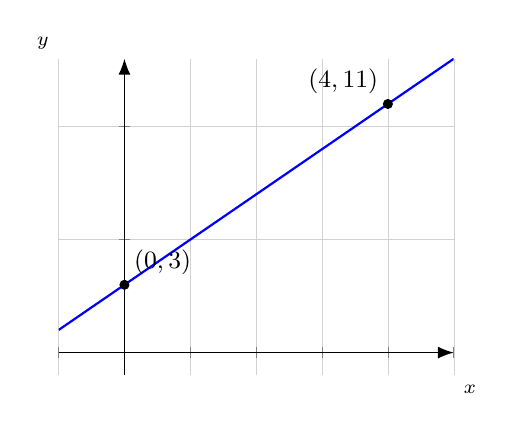
\begin{tikzpicture}
\graphaxis{-1}{5}{-1}{13}{1}
\addplot[domain=-1:5, samples=2, thick, blue] {2*x+3};
\markpt{0}{3}{above right}
\markpt{4}{11}{above left}
\end{axis}
\end{tikzpicture}
\end{center}
\qspace

\item Find the equation of the line shown.
\begin{center}
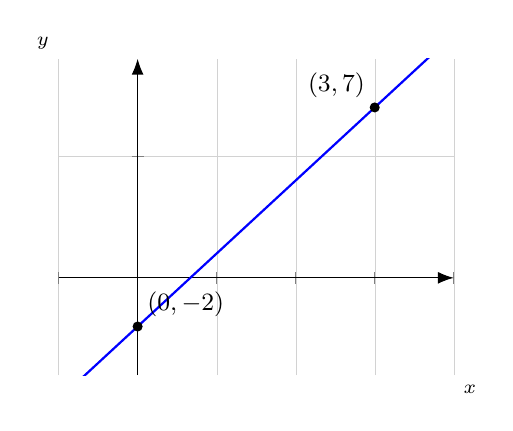
\begin{tikzpicture}
\graphaxis{-1}{4}{-4}{9}{1}
\addplot[domain=-1:4, samples=2, thick, blue] {3*x-2};
\markpt{0}{-2}{above right}
\markpt{3}{7}{above left}
\end{axis}
\end{tikzpicture}
\end{center}
\qspace

\item Find the equation of the line shown.
\begin{center}
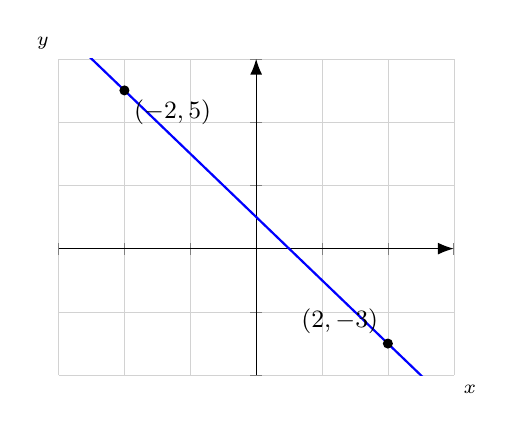
\begin{tikzpicture}
\graphaxis{-3}{3}{-4}{6}{1}
\addplot[domain=-3:3, samples=2, thick, blue] {-2*x+1};
\markpt{-2}{5}{below right}
\markpt{2}{-3}{above left}
\end{axis}
\end{tikzpicture}
\end{center}
\qspace

\item Find the equation of the line shown. The triangle marks the gradient (rise over run).
\begin{center}
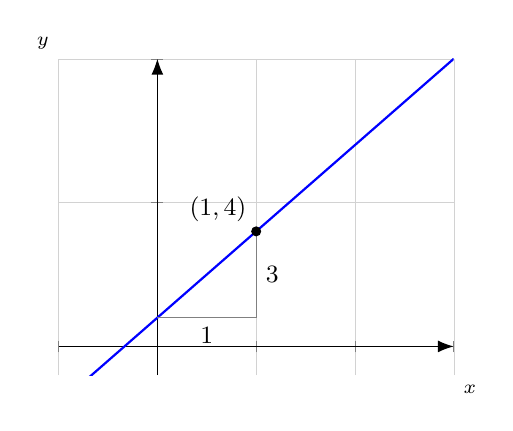
\begin{tikzpicture}
\graphaxis{-1}{3}{-1}{10}{1}
\addplot[domain=-1:3, samples=2, thick, blue] {3*x+1};
\draw[gray] (axis cs:0,1) -- (axis cs:1,1) -- (axis cs:1,4);
\node[below, font=\small] at (axis cs:0.5,1) {$1$};
\node[right, font=\small] at (axis cs:1,2.5) {$3$};
\markpt{1}{4}{above left}
\end{axis}
\end{tikzpicture}
\end{center}
\qspace

\item Find the equation of the line shown.
\begin{center}
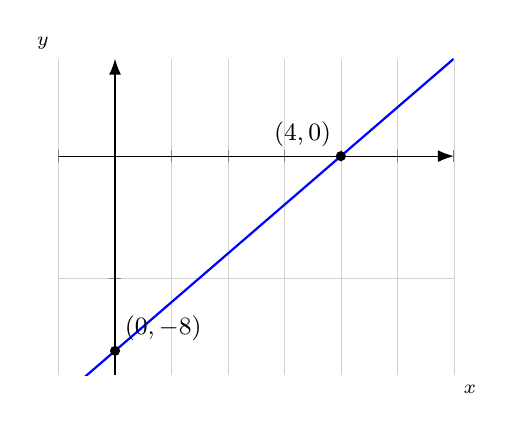
\begin{tikzpicture}
\graphaxis{-1}{6}{-9}{4}{1}
\addplot[domain=-1:6, samples=2, thick, blue] {2*x-8};
\markpt{4}{0}{above left}
\markpt{0}{-8}{above right}
\end{axis}
\end{tikzpicture}
\end{center}
\qspace

\item Find the equation of the line shown. The triangle marks the gradient (rise over run).
\begin{center}
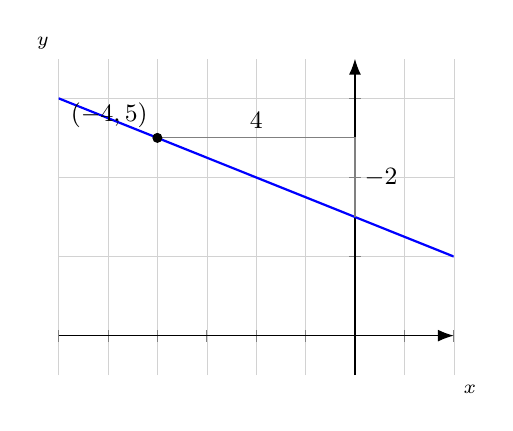
\begin{tikzpicture}
\graphaxis{-6}{2}{-1}{7}{1}
\addplot[domain=-6:2, samples=2, thick, blue] {-0.5*x+3};
\draw[gray] (axis cs:-4,5) -- (axis cs:0,5) -- (axis cs:0,3);
\node[above, font=\small] at (axis cs:-2,5) {$4$};
\node[right, font=\small] at (axis cs:0,4) {$-2$};
\markpt{-4}{5}{above left}
\end{axis}
\end{tikzpicture}
\end{center}
\qspace

\end{enumerate}

\section{Quadratics from a Turning Point}
\noindent Each graph shows the turning point and one other point. Substitute the other point into $y=a(x-h)^2+k$ to find $a$, then write the full equation.

\begin{enumerate}

\item
Find the equation of the curve shown.
\begin{center}
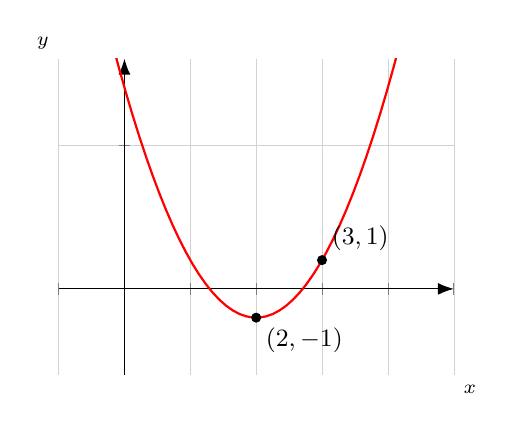
\begin{tikzpicture}
\graphaxis{-1}{5}{-3}{8}{1}
\addplot[domain=-1:5, samples=60, thick, red] {2*(x-2)^2-1};
\markpt{2}{-1}{below right}
\markpt{3}{1}{above right}
\end{axis}
\end{tikzpicture}
\end{center}
\qspace

\item
Find the equation of the curve shown.
\begin{center}
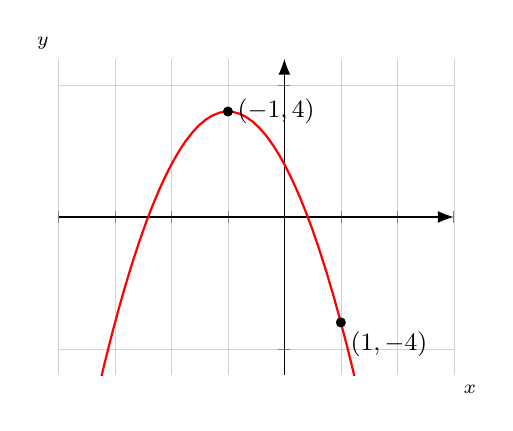
\begin{tikzpicture}
\graphaxis{-4}{3}{-6}{6}{1}
\addplot[domain=-4:3, samples=60, thick, red] {-2*(x+1)^2+4};
\markpt{-1}{4}{right}
\markpt{1}{-4}{below right}
\end{axis}
\end{tikzpicture}
\end{center}
\qspace

\item
Find the equation of the curve shown.
\begin{center}
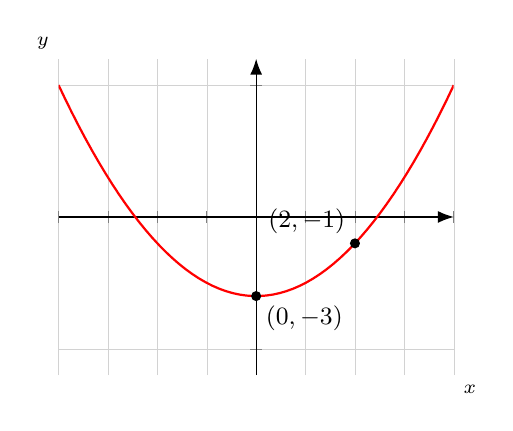
\begin{tikzpicture}
\graphaxis{-4}{4}{-6}{6}{1}
\addplot[domain=-4:4, samples=60, thick, red] {0.5*x^2-3};
\markpt{0}{-3}{below right}
\markpt{2}{-1}{above left}
\end{axis}
\end{tikzpicture}
\end{center}
\qspace

\item
Find the equation of the curve shown.
\begin{center}
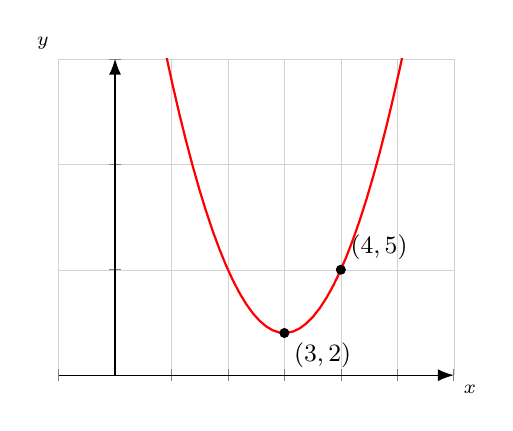
\begin{tikzpicture}
\graphaxis{-1}{6}{0}{15}{1}
\addplot[domain=-1:6, samples=60, thick, red] {3*(x-3)^2+2};
\markpt{3}{2}{below right}
\markpt{4}{5}{above right}
\end{axis}
\end{tikzpicture}
\end{center}
\qspace

\item
Find the equation of the curve shown.
\begin{center}
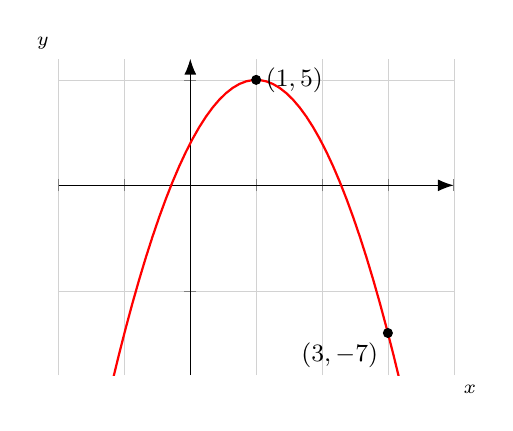
\begin{tikzpicture}
\graphaxis{-2}{4}{-9}{6}{1}
\addplot[domain=-2:4, samples=60, thick, red] {-3*(x-1)^2+5};
\markpt{1}{5}{right}
\markpt{3}{-7}{below left}
\end{axis}
\end{tikzpicture}
\end{center}
\qspace

\end{enumerate}

\section{Quadratics from Intercepts}
\noindent Each graph shows both $x$-intercepts and one other point. Substitute the other point into $y=a(x-p)(x-q)$ to find $a$, then write the full equation.

\begin{enumerate}

\item
Find the equation of the curve shown.
\begin{center}
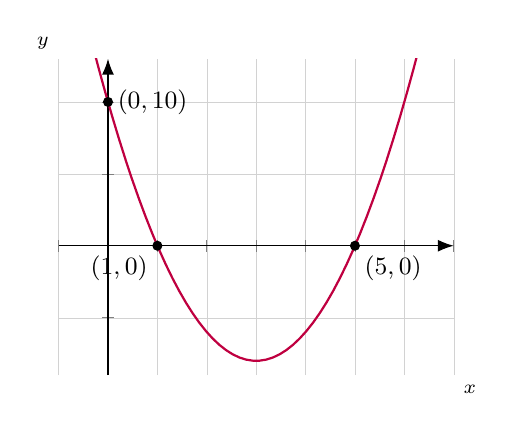
\begin{tikzpicture}
\graphaxis{-1}{7}{-9}{13}{1}
\addplot[domain=-1:7, samples=60, thick, purple] {2*(x-1)*(x-5)};
\markpt{1}{0}{below left}
\markpt{5}{0}{below right}
\markpt{0}{10}{right}
\end{axis}
\end{tikzpicture}
\end{center}
\qspace

\item
Find the equation of the curve shown.
\begin{center}
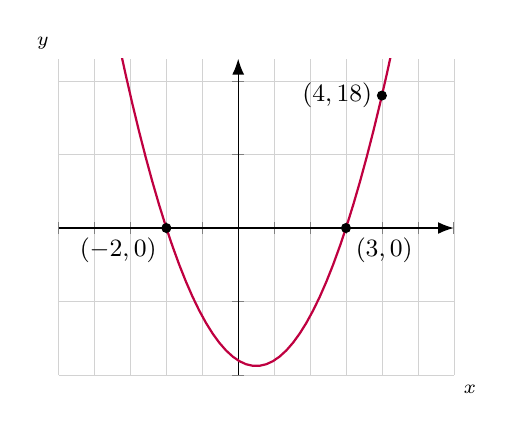
\begin{tikzpicture}
\graphaxis{-5}{6}{-20}{23}{1}
\addplot[domain=-5:6, samples=60, thick, purple] {3*(x+2)*(x-3)};
\markpt{-2}{0}{below left}
\markpt{3}{0}{below right}
\markpt{4}{18}{left}
\end{axis}
\end{tikzpicture}
\end{center}
\qspace

\item
Find the equation of the curve shown.
\begin{center}
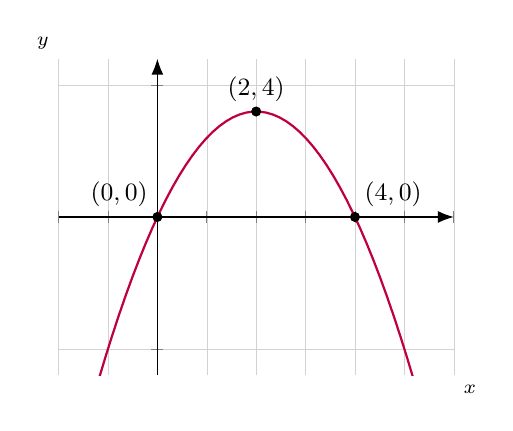
\begin{tikzpicture}
\graphaxis{-2}{6}{-6}{6}{1}
\addplot[domain=-2:6, samples=60, thick, purple] {-x*(x-4)};
\markpt{0}{0}{above left}
\markpt{4}{0}{above right}
\markpt{2}{4}{above}
\end{axis}
\end{tikzpicture}
\end{center}
\qspace

\item
Find the equation of the curve shown.
\begin{center}
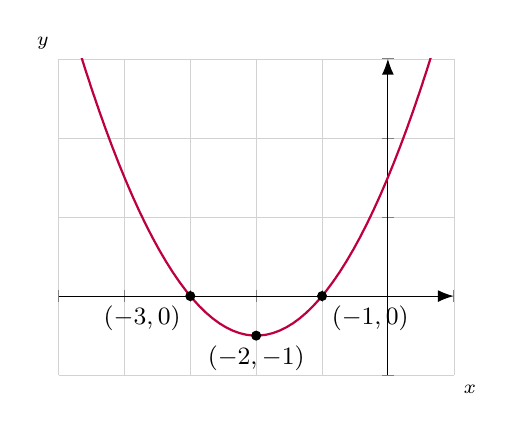
\begin{tikzpicture}
\graphaxis{-5}{1}{-2}{6}{1}
\addplot[domain=-5:1, samples=60, thick, purple] {(x+3)*(x+1)};
\markpt{-3}{0}{below left}
\markpt{-1}{0}{below right}
\markpt{-2}{-1}{below}
\end{axis}
\end{tikzpicture}
\end{center}
\qspace

\item
Find the equation of the curve shown.
\begin{center}
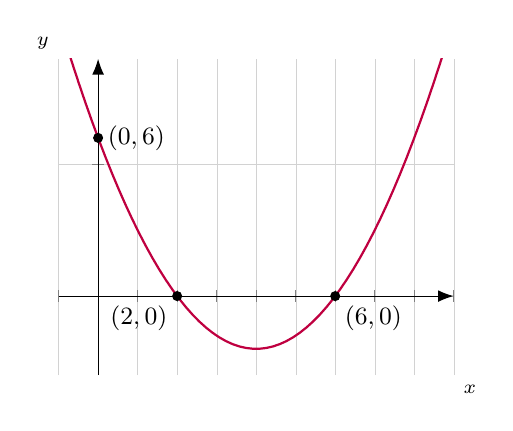
\begin{tikzpicture}
\graphaxis{-1}{9}{-3}{9}{1}
\addplot[domain=-1:9, samples=60, thick, purple] {0.5*(x-2)*(x-6)};
\markpt{2}{0}{below left}
\markpt{6}{0}{below right}
\markpt{0}{6}{right}
\end{axis}
\end{tikzpicture}
\end{center}
\qspace

\end{enumerate}

\section{Mixed Practice}
\noindent These graphs are not labelled by type. Look at what is marked --- a gradient and intercept, a turning point, or two $x$-intercepts --- to decide which form of equation to use.

\begin{enumerate}

\item
Find the equation of the graph shown.
\begin{center}
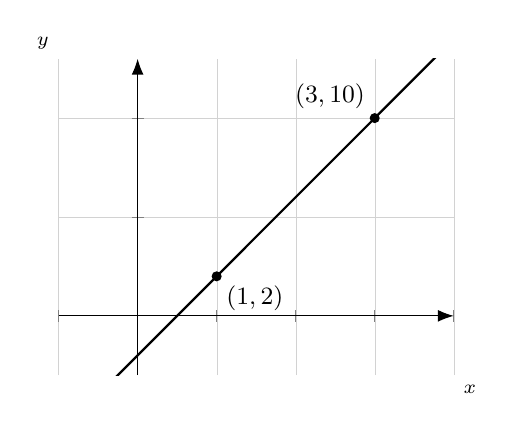
\begin{tikzpicture}
\graphaxis{-1}{4}{-3}{13}{1}
\addplot[domain=-1:4, samples=2, thick, black] {4*x-2};
\markpt{1}{2}{below right}
\markpt{3}{10}{above left}
\end{axis}
\end{tikzpicture}
\end{center}
\qspace

\item
Find the equation of the graph shown.
\begin{center}
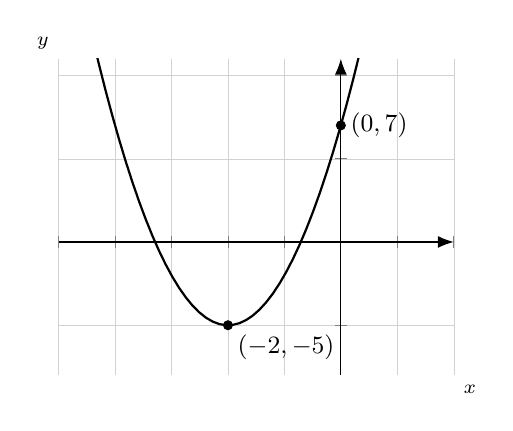
\begin{tikzpicture}
\graphaxis{-5}{2}{-8}{11}{1}
\addplot[domain=-5:2, samples=60, thick, black] {3*(x+2)^2-5};
\markpt{-2}{-5}{below right}
\markpt{0}{7}{right}
\end{axis}
\end{tikzpicture}
\end{center}
\qspace

\item
Find the equation of the graph shown.
\begin{center}
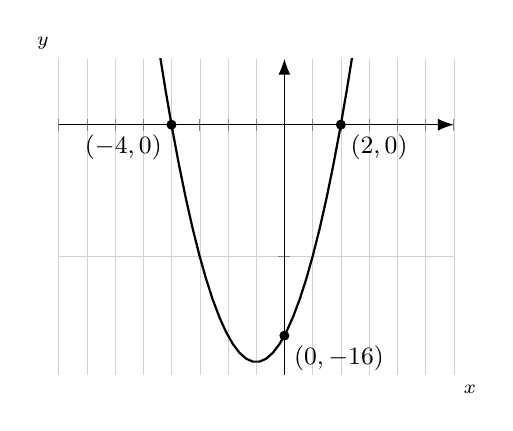
\begin{tikzpicture}
\graphaxis{-8}{6}{-19}{5}{1}
\addplot[domain=-8:6, samples=60, thick, black] {2*(x+4)*(x-2)};
\markpt{-4}{0}{below left}
\markpt{2}{0}{below right}
\markpt{0}{-16}{below right}
\end{axis}
\end{tikzpicture}
\end{center}
\qspace

\item
Find the equation of the graph shown.
\begin{center}
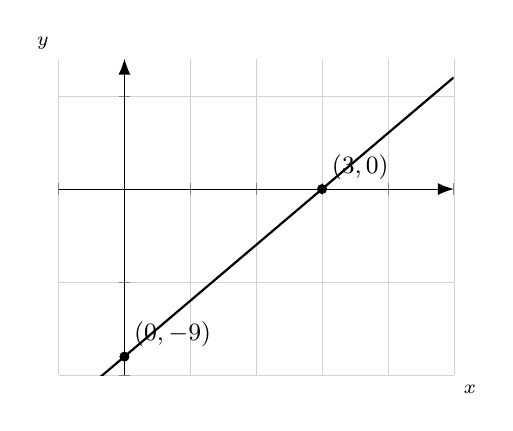
\begin{tikzpicture}
\graphaxis{-1}{5}{-10}{7}{1}
\addplot[domain=-1:5, samples=2, thick, black] {3*x-9};
\markpt{3}{0}{above right}
\markpt{0}{-9}{above right}
\end{axis}
\end{tikzpicture}
\end{center}
\qspace

\item
Find the equation of the graph shown.
\begin{center}
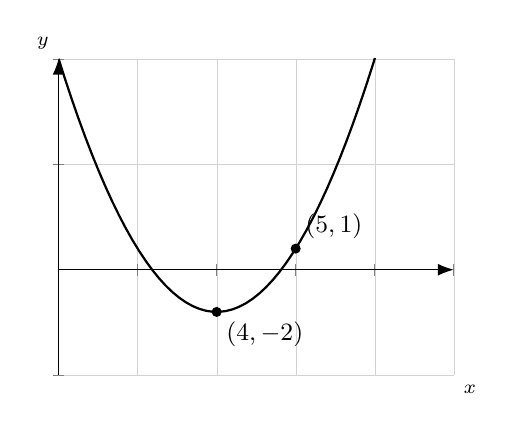
\begin{tikzpicture}
\graphaxis{2}{7}{-5}{10}{1}
\addplot[domain=2:7, samples=60, thick, black] {3*(x-4)^2-2};
\markpt{4}{-2}{below right}
\markpt{5}{1}{above right}
\end{axis}
\end{tikzpicture}
\end{center}
\qspace

\item
Find the equation of the graph shown.
\begin{center}
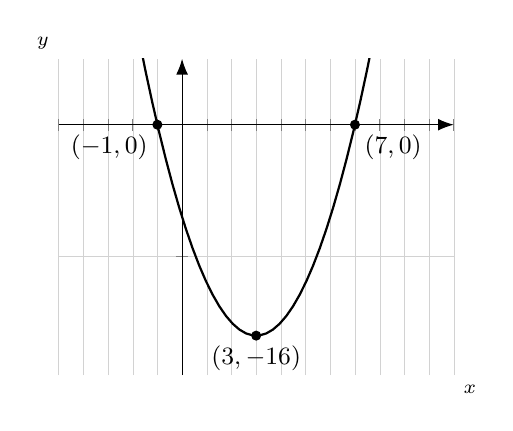
\begin{tikzpicture}
\graphaxis{-5}{11}{-19}{5}{1}
\addplot[domain=-5:11, samples=60, thick, black] {(x+1)*(x-7)};
\markpt{-1}{0}{below left}
\markpt{7}{0}{below right}
\markpt{3}{-16}{below}
\end{axis}
\end{tikzpicture}
\end{center}
\qspace

\end{enumerate}

\end{document}
